\documentclass[12pt, twoside]{article}
\usepackage[francais]{babel}
\usepackage[T1]{fontenc}
\usepackage[latin1]{inputenc}
\usepackage[left=5mm, right=5mm, top=5mm, bottom=5mm]{geometry}
\usepackage{float}
\usepackage{graphicx}
\usepackage{array}
\usepackage{multirow}
\usepackage{amsmath,amssymb,mathrsfs} 
\usepackage{soul}
\usepackage{textcomp}
\usepackage{eurosym}
\usepackage{lscape}
 \usepackage{variations}
\usepackage{tabvar}
 
\pagestyle{empty}


\begin{document}

\begin{center}
\Large{\ul{\textbf{Fonctions lin�aires}}}
\end{center}


\section{D�finitions et propri�t�s}

\ul{D�finition:} $a$ d�signe un nombre relatif. 

La \textbf{fonction lin�aire} de \textbf{coefficient} $a$ est la fonction qui,
a un nombre, associe le produit de ce nombre par $a$.

On note cette fonction: $f: x \mapsto ax$. On �crit aussi: $f(x)=ax$.

\bigskip

\ul{Exemples:}

\begin{enumerate}
  \item [$\bullet$] La fonction lin�aire $g$ de coefficient -3 se note
  
  L'image de 4 par la fonction $g$ est \ldots \ldots
  
\enskip

  \item [$\bullet$] $h: x \mapsto 5x$ est une fonction lin�aire de coefficient
\ldots  \ldots 
L'image de -1 par la fonction $h$ est \ldots \ldots

\enskip


  \item [$\bullet$] $j: x \mapsto \frac{x}{2}$ est une fonction lin�aire de coefficient
  \ldots  \ldots. On a:
$j(7)=\ldots$

\enskip

\item [$\bullet$] $f: x \mapsto x^2$ et $g: x \mapsto 2x+1$ \ldots \ldots
\ldots \ldots \ldots
\end{enumerate}


\bigskip

\ul{Propri�t�:} $f$ est une fonction lin�aire de coefficient $a$ avec $a \neq
0$. Tout nombre admet un et un seul ant�c�dent par cette fonction lin�aire.

\bigskip

\ul{Exemple:} On cherhce l'ant�c�dent de -35 par la fonction lin�aire $f$ de
coefficient 7.

La fonction $f$ est d�finie par \ldots \ldots \ldots \ldots

On cherche le nombre $x$ tel que \ldots \ldots \ldots \ldots


Donc \ldots est le seul ant�c�dent de -35 par la fonction $f$.


\section{Tableau de valeurs}


\ul{Propri�t�:} Un tableau de valeurs d'une fonction lin�aire est un tableau de
proportionnalit�.  Le coefficient de la fonction est un coefficient de
proportionnalit� de ce tableau.

\bigskip

\ul{Exemple:} $f:x \mapsto 7x$

\begin{center}
\begin{tabular}{|c|c|c|c|c|c|}
\hline
$x$ & -4 & -2 & 0 & 1 & 6 \\
\hline
$f(x)$ & \qquad & \qquad & \qquad & \qquad & \qquad \\
\hline
\end{tabular}
\end{center}


\section{Repr�sentation graphique}


\ul{Propri�t�:} Dans un rep�re, la repr�sentation graphique d'une fonction
lin�aire $f:x \mapsto ax$ est \ldots \ldots \ldots \ldots \ldots \ldots  

\bigskip

\ul{Remarques:} 

$\bullet$ Le nombre $a$ est appel� le \textbf{coefficient directeur} de
cette droite.

$\bullet$ La droite repr�sentative de la fonction $f$ passe par le point de
coordon�es $(1;a)$.


\bigskip


\ul{Exemple:} $g:x \mapsto 2x$

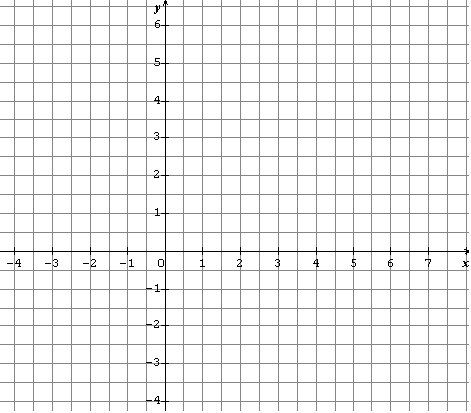
\includegraphics[width=9cm]{images/Cg.png}



\section{Pourcentages}

\ul{Propri�t�:} p d�signe un nombre positif non nul. 

\textbf{Augmenter} un nombre positif de p\% revient � multiplier ce
nombre par \big( 1+$\dfrac{p}{100}$ \big).

Une augmentation de p\% peut se traduire par la fonction lin�aire $f: x \mapsto
 (1+\dfrac{p}{100}) x$.
 
 
 \bigskip
 
 \ul{Exemple:} Un loyer de 520 \euro augmente de 1,5 \%.
 
 Le nouveau loyer est: $520 \times (1 + \dfrac{1,5}{100})=520 \times
 1,015=527,80$ \euro.
 
 
 \bigskip
 
 
\ul{Propri�t�:} p d�signe un nombre positif non nul. 

\textbf{Diminuer} un nombre positif de p\% revient � multiplier ce
nombre par \big( 1-$\dfrac{p}{100}$ \big).

Une diminution de p\% peut se traduire par la fonction lin�aire $f: x \mapsto
 (1-\dfrac{p}{100}) x$.
 
 
 \bigskip
 
 \ul{Exemple:} Un article qui coutait 125 \euro est sold� et son prix diminue
 de  35 \%.
 
 Le nouveau prix est: $125 \times (1 - \dfrac{35}{100})=125 \times
 0,65=81,25$ \euro.
 
 
 
  \bigskip
  
   \bigskip
   
 \pagebreak
 
        
        
 
 
 
\begin{tabular}{cc}
\begin{minipage}{9cm}
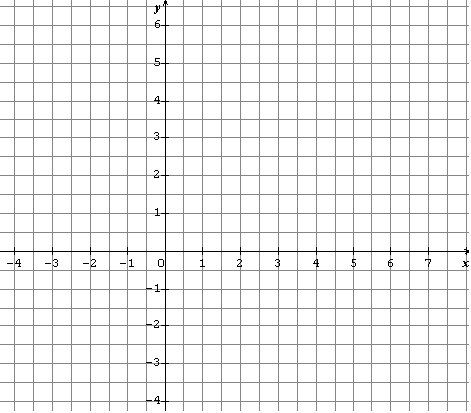
\includegraphics[width=9cm]{images/Cg.png}

\medskip

\medskip

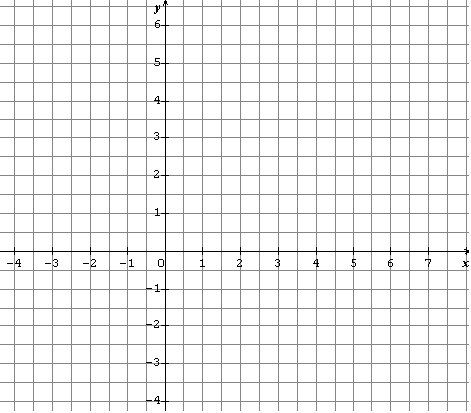
\includegraphics[width=9cm]{images/Cg.png}

\medskip

\medskip

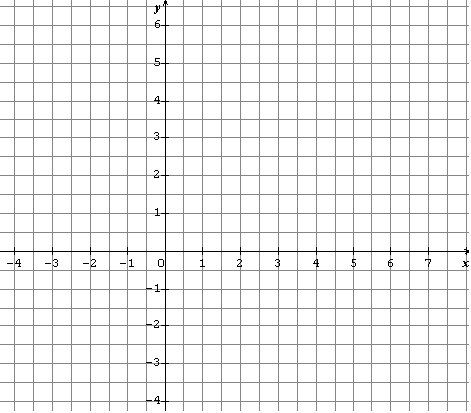
\includegraphics[width=9cm]{images/Cg.png}
\end{minipage}
&
\begin{minipage}{9cm}
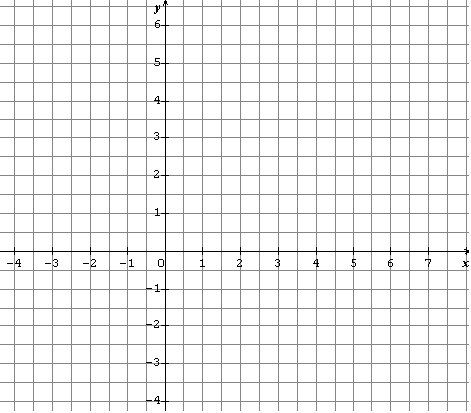
\includegraphics[width=9cm]{images/Cg.png}

\medskip

\medskip

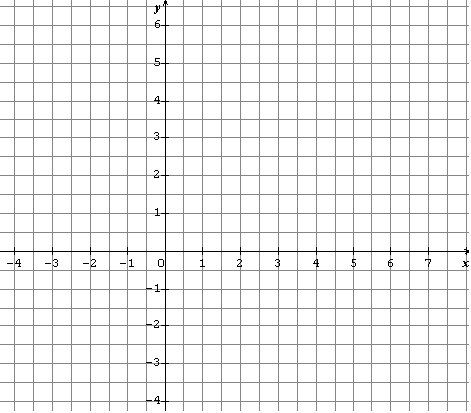
\includegraphics[width=9cm]{images/Cg.png}

\medskip


\medskip

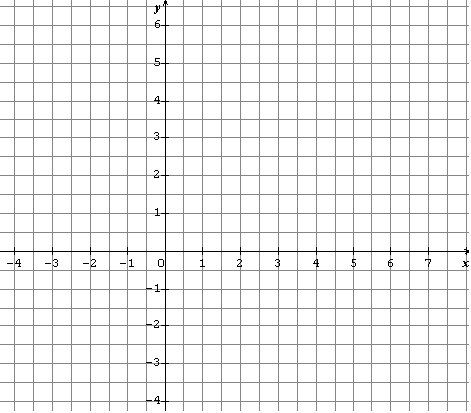
\includegraphics[width=9cm]{images/Cg.png}
\end{minipage}
\end{tabular}







\end{document}
